\documentclass[10pt]{article}
\usepackage[paperwidth=9in,paperheight=16in,margin=0in]{geometry}
\usepackage{tikz}
\usepackage{xcolor}
\usepackage{lmodern}
\usepackage{sfmath}
\pagestyle{empty}

\usetikzlibrary{arrows.meta,positioning,fit,calc}

\begin{document}
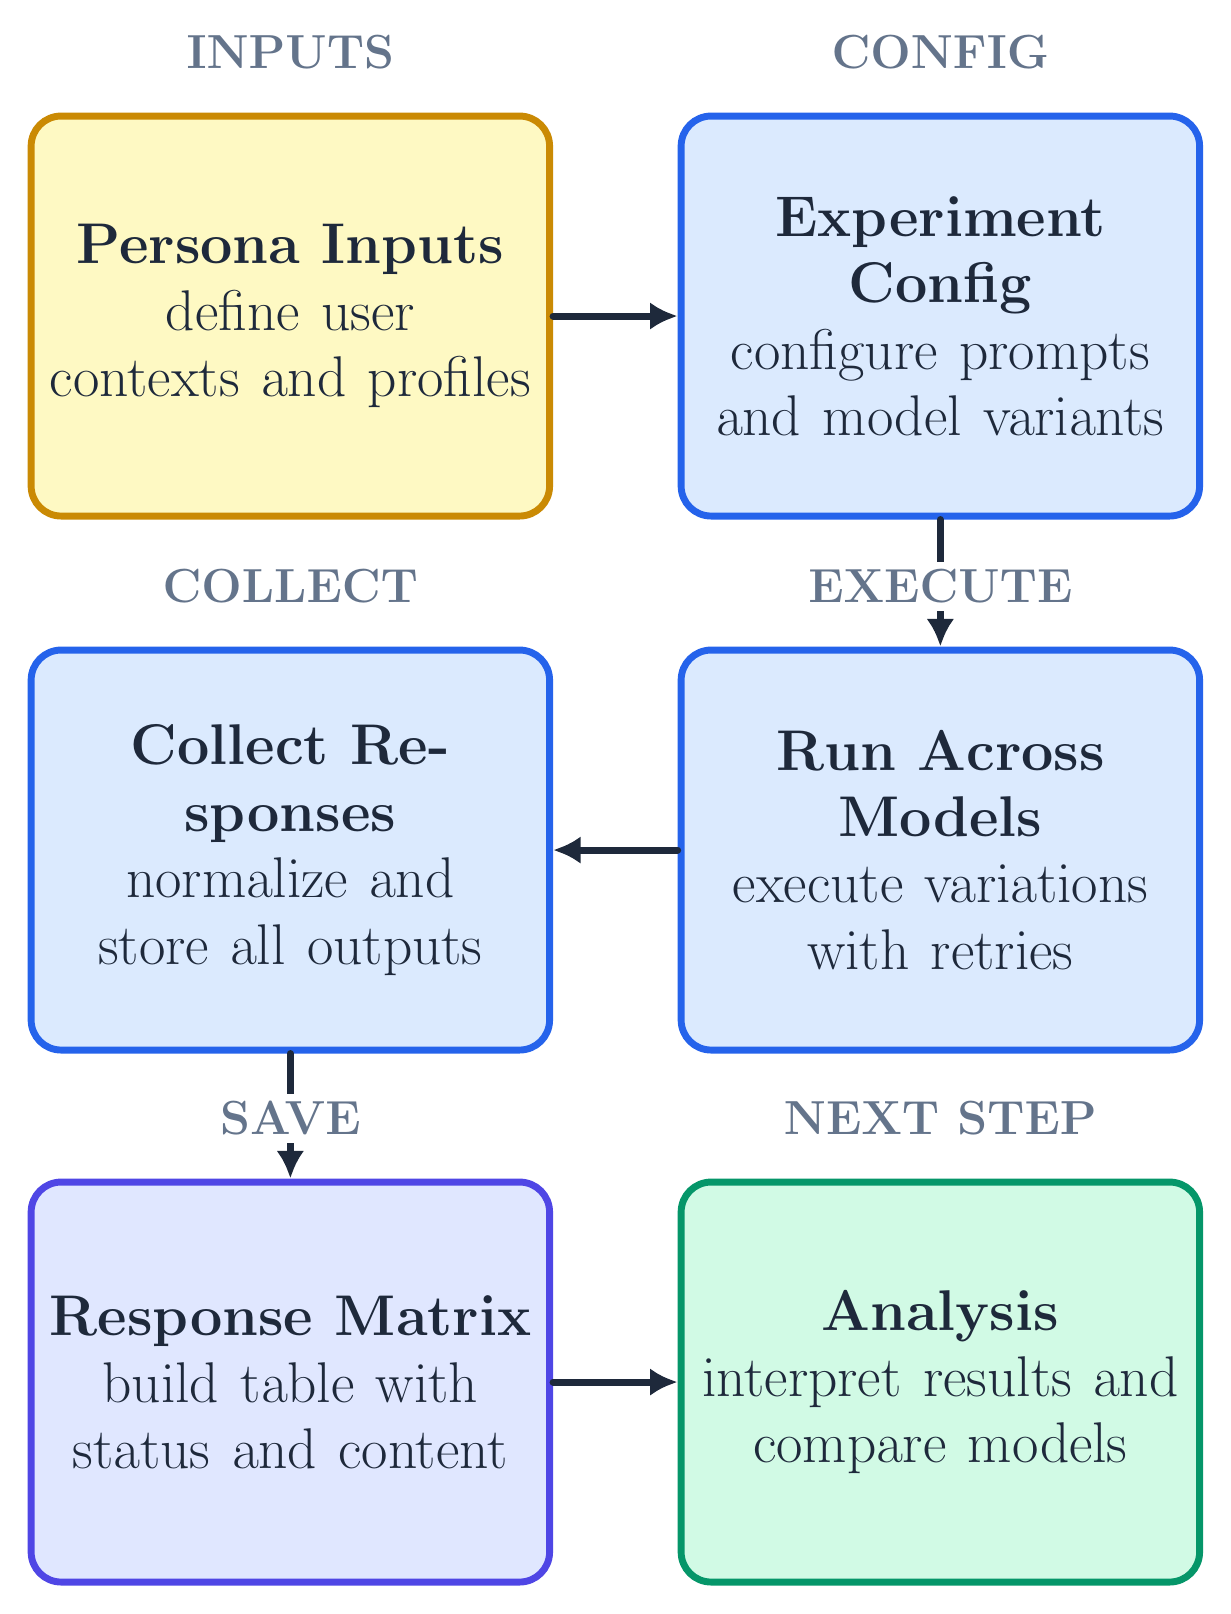
\begin{tikzpicture}[x=1in,y=1in]

	% ============================================================
	% COLORS
	% ============================================================
	\definecolor{text}{HTML}{1E293B}
	\definecolor{muted}{HTML}{64748B}
	\definecolor{startFill}{HTML}{FEF9C3}
	\definecolor{startStroke}{HTML}{CA8A04}
	\definecolor{coreFill}{HTML}{DBEAFE}
	\definecolor{coreStroke}{HTML}{2563EB}
	\definecolor{matrixFill}{HTML}{E0E7FF}
	\definecolor{matrixStroke}{HTML}{4F46E5}
	\definecolor{finishFill}{HTML}{D1FAE5}
	\definecolor{finishStroke}{HTML}{059669}

	% ============================================================
	% STYLES
	% ============================================================
	\tikzset{
		box/.style={
			rounded corners=0.15in,
			minimum width=2.5in,
			minimum height=2.0in,
			text width=2.5in,
			align=center,
			font=\bfseries\fontsize{20}{24}\selectfont,
			text=text,
			line width=2.5pt
		},
	startBox/.style={box, fill=startFill, draw=startStroke},
	coreBox/.style={box, fill=coreFill, draw=coreStroke},
	matrixBox/.style={box, fill=matrixFill, draw=matrixStroke},
	finishBox/.style={box, fill=finishFill, draw=finishStroke},
	arr/.style={-{Latex[length=10pt,width=10pt]},line width=2.5pt,draw=text,line cap=round,line join=round},
	lbl/.style={font=\bfseries\fontsize{16}{18}\selectfont,text=muted,fill=white,inner sep=3pt,outer sep=2pt}
	}

	% ============================================================
	% LAYOUT - 3x2 GRID SERPENTINE (portrait 9:16)
	% ============================================================
	% Canvas: 9x16 (portrait)
	% Flow: Inputs -> Config -> Run -> Collect -> Matrix -> Insight
	% Columns: x=2.50 (left), x=6.50 (right) - gap=4in
	% Rows: y=13.00, 8.00, 3.00

	% ROW 1
	\node[startBox] (input)  at (2.50, 13.00) {Persona Inputs\\\mdseries define user\\contexts and profiles};
	\node[coreBox]  (config) at (5.75, 13.00) {Experiment\\Config\\\mdseries configure prompts and model variants};

	% ROW 2
	\node[coreBox]  (run)    at (5.75, 10.33) {Run Across Models\\\mdseries execute variations\\with retries};
	\node[coreBox]  (collect) at (2.50, 10.33) {Collect Responses\\\mdseries normalize and store all outputs};

	% ROW 3
	\node[matrixBox] (matrix)  at (2.50, 7.67) {Response Matrix\\\mdseries build table with status and content};
	\node[finishBox] (insight) at (5.75, 7.67) {Analysis\\\mdseries interpret results and compare models};

	% ============================================================
	% ARROWS - ROW 1 (L to R)
	% ============================================================
	\draw[arr] (input.east) -- (config.west);

	% ============================================================
	% ARROWS - ROW 2 (R to L: Run -> Collect)
	% ============================================================
	\draw[arr] (run.west) -- (collect.east);

	% ============================================================
	% ARROWS - ROW 3 (L to R: Matrix -> Insight)
	% ============================================================
	\draw[arr] (matrix.east) -- (insight.west);

	% ============================================================
	% ARROWS - VERTICAL CONNECTORS
	% ============================================================
	\draw[arr] (config.south) -- (run.north);
	\draw[arr] (collect.south) -- (matrix.north);

	% ============================================================
	% PHASE LABELS
	% ============================================================
	\node[lbl, anchor=south, yshift=0.15in] at (input.north)   {INPUTS};
	\node[lbl, anchor=south, yshift=0.15in] at (config.north)  {CONFIG};
	\node[lbl, anchor=south, yshift=0.15in] at (run.north)    {EXECUTE};
	\node[lbl, anchor=south, yshift=0.15in] at (collect.north) {COLLECT};
	\node[lbl, anchor=south, yshift=0.15in] at (matrix.north)  {SAVE};
	\node[lbl, anchor=south, yshift=0.15in] at (insight.north) {NEXT STEP};

\end{tikzpicture}
\end{document}